%! TEX root = ../main.tex
\documentclass[main]{subfiles}

\begin{document}

\chapter{考察}
\section{重さ}
カーリングをプレイするにあたって,カーラングブラシを使用するほどブラシパッドに氷上のゴミが付着していくのでゴ
ミの分の質量が増加するように考えられるが,実際の結果では使用期間が長いほど質量は減っていた.これは付着して増
えたゴミの質量よりもブラシパッドを使用して摩耗して擦り切れていった繊維の質量のほうが多いと言える.
\\

\section{表面の繊維}
低倍率で比較したときに使用期間が長いものほどゴミの付着量が多いことがわかるが,高倍率で見ると繊維が擦り切れて
細くなっているものがあった.また,色が薄くなっており,繊維と繊維の隙間が大きくなっていることから,密度が小さく
なっていることが言える.

実験結果からスイープ方向に垂直に並んでいる繊維がパッドの役割を果たしているものだと考えられる.未使用のものは繊維が
隙間なく並んでいるが長期間使用したものは繊維がバラバラに分かれてしまっている部分もあり,未使用のものと同じ性能を発揮
できるとは言えない.

10~15投使用したものはサンプルAとサンプルBで摩耗具合が違った.サンプルBのほうが摩耗していた理由としては,使用する
際にブラシパッドのもつ向きが偏っていたことが考えられる,

\begin{figure}[htbp]
    \centering
    \begin{minipage}[htbp]{0.3\linewidth}
        \centering
        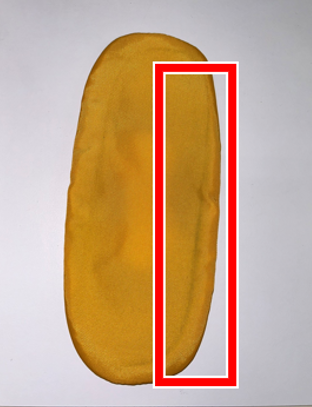
\includegraphics[keepaspectratio, width=0.8\linewidth, height=\linewidth]{figures/caring_brush_pad/10~15Akousatu.png}
        \caption{10~15投使用A}
        \label{fig:label}
    \end{minipage}
    \begin{minipage}[htbp]{0.3\linewidth}
        \centering
        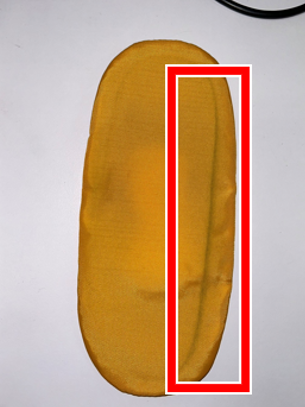
\includegraphics[keepaspectratio, width=0.8\linewidth, height=\linewidth]{figures/caring_brush_pad/10~15Bkousatu.png}
        \caption{10~15投使用B}
        \label{fig:label}
    \end{minipage}
\end{figure}

サンプルAとサンプルBを比較したときにサンプルBはサンプルAよりもブラシパッドの右側が汚く,左側は未使用のものの
ように綺麗であることがわかる.このことから何投か使用した後にブラシパッドの倒す方向を逆にすることで使用感が
良い状態を少しではあるが長持ちさせることができると言える.
\\

\section{色の違い}

dgadfa

\end{document}